\documentclass[11pt]{article}

%% ---- Layout ----
\usepackage[a4paper,margin=1in]{geometry}
\usepackage{parskip}

%% ---- Math ----
\usepackage{amsmath}
\usepackage{amssymb}
\usepackage{amsthm}
\usepackage{mathtools}    % \coloneqq, \DeclarePairedDelimiter, etc.
\usepackage{bm}

%% ---- Bibliography (natbib for \citep) ----
\usepackage[round,authoryear]{natbib}

%% ---- Algorithms ----
\usepackage{algorithm}
\usepackage{algpseudocode}
\algnewcommand\algorithmicforeach{\textbf{for each}}
\algdef{S}[FOR]{ForEach}[1]{\algorithmicforeach\ #1\ \algorithmicdo}

%% ---- Figures ----
\usepackage{graphicx}
\usepackage{caption}
\usepackage{subcaption}

%% ---- Cross-references ----
\usepackage{hyperref}
\usepackage{cleveref}

%% ---- Theorem environments ----
\theoremstyle{plain}
\newtheorem{theorem}{Theorem}
\newtheorem{proposition}[theorem]{Proposition}
\newtheorem{corollary}[theorem]{Corollary}

\theoremstyle{definition}
\newtheorem{definition}[theorem]{Definition}

\theoremstyle{remark}
\newtheorem{remark}[theorem]{Remark}

\title{Theory: 2D BarDistribution, mixture MALC,\\
       optimal-transport aggregation, and variance reduction}
\author{}
\date{}

\begin{document}
\maketitle

%% =============================================================================
%% Consolidated theoretical section for the CFM / R-PFN paper.
%%
%% Contents (in intended reading order):
%%   1. Two-dimensional \texttt{BarDistribution} head          (Sec. \ref{sec:2d-bardistribution})
%%   2. Multimodal density recovery with MALC                  (Sec. \ref{sec:malc-multimodal})
%%   3. Population aggregation via the 2-Wasserstein barycenter (Sec. \ref{sec:ot-barycenter})
%%   4. Variance reduction of the joint estimator              (Sec. \ref{sec:variance-reduction})
%%
%% All theorem-level statements are limited to results we can either verify
%% directly (variance-formula computations, definitions in the source) or
%% cite (Agueh-Carlier, Cule-Samworth-Stewart, Sheppard).
%% =============================================================================


%% -----------------------------------------------------------------------------
\subsection{Two-dimensional \texttt{BarDistribution} head}
\label{sec:2d-bardistribution}

Our model outputs a density over the paired potential outcomes
$(Y_{\mathrm{do}(0)}, Y_{\mathrm{do}(1)})$ using a two-dimensional
extension of UWYK's \texttt{BarDistribution} head. All quantities below
are conditional on the query covariate $X$ and the observational
context; we suppress that conditioning for readability.

\paragraph{Domain and bin structure.}
Observed outcomes are min--max scaled to $[-1, 1]$ using the context
range. The interior domain $\mathcal{I} \coloneqq [-1,1]^{2}$ is
partitioned into a uniform $K \times K$ grid of bins with bin width
$h \coloneqq 2/K$ per axis. We write $B_{j_0, j_1}$ for the bin whose
lower-left corner is $\bigl(-1 + j_0 h,\, -1 + j_1 h\bigr)$, so
$B_{j_0, j_1}$ has area $h^{2}$ and
$\bigcup_{j_0, j_1} B_{j_0, j_1} = \mathcal{I}$.

\paragraph{Per-query output.}
For each query the model emits $K^{2} + 9 + 4$ logits:
\begin{itemize}
  \item \emph{Inner logits} $\ell \in \mathbb{R}^{K^{2}}$ pass through a
    softmax to give the discrete joint
    \begin{equation}
      p_{j_0, j_1} \;=\;
      \frac{\exp(\ell_{j_0, j_1})}
           {\sum_{i_0, i_1} \exp(\ell_{i_0, i_1})},
      \qquad
      \sum_{j_0, j_1} p_{j_0, j_1} = 1.
      \label{eq:pmat-softmax}
    \end{equation}
  \item \emph{Region logits} $u \in \mathbb{R}^{9}$ pass through a
    softmax to give the mixture weights $w \in \Delta^{8}$ over the nine
    regions defined below:
    \begin{equation}
      w_r \;=\; \frac{\exp(u_r)}{\sum_{s=1}^{9} \exp(u_s)},
      \qquad r \in \{1, \dots, 9\}.
      \label{eq:region-weights}
    \end{equation}
  \item \emph{Raw tail parameters}
    $(\sigma_{L}^{(0)\text{raw}}, \sigma_{R}^{(0)\text{raw}},
      \sigma_{L}^{(1)\text{raw}}, \sigma_{R}^{(1)\text{raw}})$
    are transformed to positive scales via softplus with a small floor
    $\varepsilon > 0$:
    \begin{equation}
      \sigma_{d}^{(\ell)} \;=\; h \cdot
      \bigl(\mathrm{softplus}\bigl(\sigma_{d}^{(\ell)\text{raw}}\bigr)
            + \varepsilon\bigr),
      \qquad d \in \{L, R\},\; \ell \in \{0, 1\}.
      \label{eq:tail-scales}
    \end{equation}
\end{itemize}

\paragraph{Three-region density.}
The full density $f(y_0, y_1)$ is defined piecewise according to where
$(y_0, y_1)$ falls relative to $\mathcal{I}$. Let
$\mathrm{IN}(y) \coloneqq \mathbf{1}\{y \in [-1, 1]\}$.
The nine mutually exclusive regions are grouped into three cases.

\subparagraph{Case 1 --- inner$\times$inner.}
If $\mathrm{IN}(y_0) = \mathrm{IN}(y_1) = 1$, the discrete grid
\eqref{eq:pmat-softmax} defines a piecewise-constant density on
$\mathcal{I}$:
\begin{equation}
  f_{\mathrm{inner}}(y_0, y_1)
  \;=\;
  \frac{p_{j_0(y_0),\, j_1(y_1)}}{h^{2}},
  \qquad
  j_\ell(y) \coloneqq \bigl\lfloor (y + 1)/h \bigr\rfloor.
  \label{eq:inner-density}
\end{equation}
Both the assignment $j_\ell(\cdot)$ and the softmax weights
\eqref{eq:pmat-softmax} are differentiable in $\ell$.

\subparagraph{Case 2 --- mixed (one inside, one outside).}
Assume $y_0 \in [-1, 1]$ and $y_1 < -1$ (the other three mixed
subcases are symmetric). We factor
\begin{equation}
  f_{\mathrm{mix}}(y_0, y_1)
  \;=\;
  p_{L}^{(1)}(y_1)\, \cdot\, g(y_0 \mid y_1 = -1),
  \label{eq:mix-density}
\end{equation}
where the tail contribution
\begin{equation}
  p_{L}^{(1)}(y_1)
  \;=\;
  \frac{2}{\sigma_{L}^{(1)}}\,
  \phi\!\left(\tfrac{y_1 - (-1)}{\sigma_{L}^{(1)}}\right)
\end{equation}
is a scaled half-Gaussian on $(-\infty, -1]$ ($\phi$ is the standard
normal density) and
\begin{equation}
  g(y_0 \mid y_1 = -1)
  \;=\;
  \frac{p_{j_0(y_0),\, 0}}
       {\bigl(\sum_{i_0} p_{i_0,\, 0}\bigr) \cdot h}
  \label{eq:boundary-conditional}
\end{equation}
is the discrete boundary conditional obtained by evaluating $p$ on the
$y_1$-most row and renormalising over the in-range axis. The
approximation
$p(y_0 \mid y_1 < -1) \approx p(y_0 \mid y_1 = -1)$
is a modelling choice justified in
\S\ref{sec:2d-bardistribution:notes} below.

\subparagraph{Case 3 --- both outside.}
If both coordinates are outside $[-1, 1]$, we use a bivariate
half-Gaussian truncated to the appropriate quadrant. Fixing signs
$(s_0, s_1) \in \{L, R\}^{2}$ that select the quadrant, the density is
\begin{equation}
  f_{\mathrm{tail}}(y_0, y_1)
  \;=\;
  \frac{1}{Z(s_0, s_1,\rho)}\,
  \phi_{2}\!\left(\tilde{y}_0, \tilde{y}_1;\, \rho\right),
  \qquad
  \tilde{y}_\ell = \frac{y_\ell - c_\ell}{\sigma_{s_\ell}^{(\ell)}},
  \label{eq:tail-density}
\end{equation}
where $c_\ell \in \{-1, +1\}$ is the corresponding boundary,
$\phi_{2}(\cdot,\cdot;\rho)$ is the standard bivariate normal density
with correlation $\rho$, and $Z(s_0, s_1, \rho)$ is the quadrant
probability given by Sheppard's identity
\citep{sheppard1899application}:
\begin{equation}
  Z(s_0, s_1, \rho)
  \;=\;
  \begin{cases}
    \tfrac{1}{4} + \tfrac{\arcsin\rho}{2\pi}
      & \text{if } s_0 = s_1, \\[4pt]
    \tfrac{1}{4} - \tfrac{\arcsin\rho}{2\pi}
      & \text{if } s_0 \ne s_1.
  \end{cases}
  \label{eq:sheppard}
\end{equation}

\paragraph{Correlation derived from the histogram.}
The correlation $\rho$ used in
\eqref{eq:tail-density}--\eqref{eq:sheppard} is not a separate learned
parameter. It is the Pearson correlation of the discrete distribution
$\{p_{j_0, j_1}\}$ evaluated at bin midpoints
$m_\ell(j_\ell) \coloneqq -1 + h\bigl(j_\ell + \tfrac{1}{2}\bigr)$:
\begin{equation}
\begin{aligned}
\bar{y}_\ell \;&=\; \sum_{j_0, j_1} p_{j_0, j_1}\, m_\ell(j_\ell), \\
v_\ell \;&=\; \sum_{j_0, j_1} p_{j_0, j_1}
             \bigl(m_\ell(j_\ell) - \bar{y}_\ell\bigr)^{2}, \\
c \;&=\; \sum_{j_0, j_1} p_{j_0, j_1}
        \bigl(m_0(j_0) - \bar{y}_0\bigr)
        \bigl(m_1(j_1) - \bar{y}_1\bigr), \\
\rho \;&=\; \frac{c}{\sqrt{v_0\, v_1} + \varepsilon}.
\end{aligned}
\label{eq:rho-derived}
\end{equation}
Deriving $\rho$ from $p$ removes one degree of freedom and ensures the
correlation that governs the tail Gaussians is the same one implicit in
the inner histogram.

\paragraph{Unified density and loss.}
The joint density at any $(y_0, y_1) \in \mathbb{R}^{2}$ is the mixture
\begin{equation}
  f(y_0, y_1)
  \;=\;
  w_{1}\, f_{\mathrm{inner}}(y_0, y_1)
  \;+\!\sum_{r = 2}^{5}\! w_{r}\, f^{(r)}_{\mathrm{mix}}(y_0, y_1)
  \;+\!\sum_{r = 6}^{9}\! w_{r}\, f^{(r)}_{\mathrm{tail}}(y_0, y_1),
  \label{eq:full-density}
\end{equation}
where the four mixed and four tail components correspond to the four
directional orientations described above. Because the nine regions
partition $\mathbb{R}^{2}$, at any query point exactly one region
component is nonzero. The training loss on a labelled point
$(y_0^\star, y_1^\star)$ is the negative log-density
\begin{equation}
  \mathcal{L}(y_0^\star, y_1^\star)
  \;=\;
  -\log\, f(y_0^\star, y_1^\star),
  \label{eq:nll}
\end{equation}
averaged over queries in a batch. In the inner-inner case
\eqref{eq:inner-density}, $\log f$ carries an explicit $-\log h^{2}$
correction relative to plain cross-entropy over the discrete grid; this
correction is required for the loss to be a proper log-density on the
continuous domain.

\paragraph{Notes on the mixed-case approximation.}
\label{sec:2d-bardistribution:notes}
The mixed density \eqref{eq:mix-density} approximates
$p(y_0 \mid y_1 < -1)$ by the boundary conditional
$p(y_0 \mid y_1 = -1)$. This is exact only when
$Y_0 \perp\!\!\!\perp Y_1$; more generally it introduces error whose
magnitude is controlled by the local variation of $p(y_0 \mid y_1)$
across the tail. The half-Gaussian factor assigns exponentially
decreasing mass to values of $y_1$ far from the boundary, so the
approximation contributes most weight where it is most accurate. We do
not claim asymptotic exactness; the choice is a bias--variance trade-off
motivated by keeping the loss differentiable and $\mathcal{O}(1)$
per-query.


%% -----------------------------------------------------------------------------
\subsection{Multimodal density recovery via mixture MALC}
\label{sec:malc-multimodal}

The training-time head outputs the discrete grid
$\{p_{j_0, j_1}\}$ of Eq.~\eqref{eq:pmat-softmax}, which is a
piecewise-constant density on $\mathcal{I}$. To recover a smooth
density we build on the mean-adjusted log-concave (MALC) estimator of
\citet{danisman2026malc}: MALC produces a shape-constrained
nonparametric density estimate from grouped (binned) probabilities
without bandwidth selection. Because a single log-concave density is
unimodal by construction, we extend MALC to a $K$-component mixture in
order to represent the multimodal joints that arise in causal
inference under posterior uncertainty over compatible SCMs.

\paragraph{Base class: 2D log-concave densities.}
A density $f: \mathbb{R}^{2} \to \mathbb{R}_{\ge 0}$ is
\emph{log-concave} if $\log f$ is concave (with the convention
$\log 0 = -\infty$). This is a nonparametric shape-constrained class
that contains all Gaussians, exponentials, uniform distributions on
convex sets, and any density with concave log; every log-concave
density is unimodal.
For any set of samples $y_1, \dots, y_M \in \mathbb{R}^{2}$ in general
position, the (nonparametric) log-concave MLE
\begin{equation}
  \hat{f}_{\mathrm{LC}}
  \;=\;
  \arg\!\max_{f \in \mathcal{F}_{\mathrm{LC}}}
  \;\;\frac{1}{M}\sum_{m=1}^{M} \log f(y_m)
  \label{eq:lc-mle}
\end{equation}
exists uniquely and is piecewise log-linear on a triangulation of the
sample support \citep{cule2010maximum,samworth2018recent}.

\paragraph{Single-component MALC from grouped data.}
Direct application of \eqref{eq:lc-mle} would require raw samples,
which the head does not produce; the head emits only the bin
probabilities $\{p_{j_0, j_1}\}$. MALC handles exactly this case by
first correcting for within-bin mass misalignment before applying the
log-concave MLE \citep{danisman2026malc}. Concretely, MALC executes
the four steps recorded in the code and its accompanying
\texttt{SUMMARY.md}:
(i) a truncated-normal fixed-point iteration recovers a latent mean per
axis from the binned marginals; (ii) a Beta jitter distribution is
calibrated so its per-axis mean matches (i); (iii) $B$ synthetic
sample points are drawn by sampling bins from $p$ with jitter within
each sampled bin; (iv) the 2D log-concave MLE \eqref{eq:lc-mle} is fit
on the $B$ synthetic points. We refer to \citet{danisman2026malc} for
the theoretical properties of the estimator and its behaviour under
grid refinement. We denote a single MALC component
$\hat{f} \in \mathcal{F}_{\mathrm{LC}}$.

\paragraph{Mixture MALC ($K$ components).}
Because $\mathcal{F}_{\mathrm{LC}}$ is unimodal, a single MALC fit
cannot represent the multimodal joints that arise when the posterior
concentrates on multiple compatible SCMs
(Section~\ref{sec:mixture-scm}). We therefore consider the mixture
family
\begin{equation}
  \mathcal{F}_{\mathrm{MALC}}^{(K)}
  \;=\;
  \Big\{\,
    f \;=\; \sum_{k=1}^{K} \pi_k\, f_k
    \;:\;
    \pi \in \Delta^{K-1},\;\;
    f_k \in \mathcal{F}_{\mathrm{LC}}\;\;\forall k
  \,\Big\},
  \label{eq:malc-family}
\end{equation}
where each $f_k$ is a single-component MALC estimator obtained by the
procedure above. Membership in $\mathcal{F}_{\mathrm{MALC}}^{(K)}$
permits up to $K$ distinct modes while retaining the shape constraint
within each component.

\paragraph{Mixture EM.}
For a fixed $K > 1$, components are combined via expectation--maxi\-mi\-sa\-tion
on the binned data. Let $\gamma_{j_0 j_1, k}^{(t)}$ denote the
responsibility of component $k$ for bin $(j_0, j_1)$ at iteration $t$,
and let $F_k^{(t)}(j_0, j_1) \coloneqq \int_{B_{j_0, j_1}} f_k^{(t)}$
denote the bin-integrated component density. The two updates are
\begin{align}
  \gamma_{j_0 j_1, k}^{(t+1)}
  \;&=\;
  \frac{\pi_k^{(t)}\, F_k^{(t)}(j_0, j_1)}
       {\sum_{j} \pi_j^{(t)}\, F_j^{(t)}(j_0, j_1)},
  \label{eq:malc-estep}
  \\[2pt]
  \pi_k^{(t+1)}
  \;&=\;
  \sum_{j_0, j_1} p_{j_0, j_1}\, \gamma_{j_0 j_1, k}^{(t+1)},
  \label{eq:malc-pi-update}
  \\[2pt]
  f_k^{(t+1)}
  \;&=\;
  \text{single-component refit on }
  \{p_{j_0, j_1}\, \gamma_{j_0 j_1, k}^{(t+1)}\}.
  \label{eq:malc-mstep}
\end{align}
Initialisation is a Voronoi assignment around modal peaks detected on
$p$ (with a deterministic augmentation when $K$ exceeds the number of
detected peaks); the iterations stop after five consecutive non-improving
log-likelihoods.

\paragraph{Algorithmic summary.}
Algorithm~\ref{alg:malc-mixture} collects the mixture EM iterations
described above and the BIC-based order selection described below into
a single pipeline. Only the outer BIC loop and the inner refit at
$K^\star$ vary between the "scan" and "final" stages; both stages
reuse the same component-fit and E-/M-step primitives.

\begin{algorithm}[t]
\caption{Mixture MALC from binned probabilities $\{p_{j_0, j_1}\}$.}
\label{alg:malc-mixture}
\begin{algorithmic}[1]
\Require Binned joint $\{p_{j_0, j_1}\}$ on a $K_g \times K_g$ grid;
maximum order $K_{\max}$; synthetic-sample size $B$; patience $\Pi$.
\Ensure Multimodal density estimate
$\hat{p}_{\mathrm{MALC}} = \sum_{k} \hat\pi_k^\star \hat f_k^\star$.
\Function{FitComponent}{$w_{j_0, j_1}$}\Comment{single MALC on a weighted grid}
    \State $\hat\mu_\ell \gets$ truncated-normal fixed-point mean per axis
    \State $\alpha, \beta \gets$ Beta-jitter parameters calibrated so
        $\mathbb{E}[\text{Beta}] = \hat\mu_\ell$
    \State draw $B$ bin indices $\{(j_0^b, j_1^b)\}_{b=1}^{B}$ from $w$
    \State $y_b \gets \text{bin midpoint of }(j_0^b, j_1^b) + \text{jitter}(\alpha, \beta)$
    \State \Return log-concave MLE \eqref{eq:lc-mle} on $\{y_b\}$
\EndFunction
\For{$K \in \{1, \dots, K_{\max}\}$}
    \State detect modal peaks of $p$; assign each bin to nearest peak via Voronoi \Comment{init}
    \ForEach{$k \in \{1, \dots, K\}$}
        \State $f_k^{(0)} \gets \Call{FitComponent}{p \cdot \mathbf{1}\{\text{bin} \in \text{Voronoi cell } k\}}$
        \State $\pi_k^{(0)} \gets $ prior mass in Voronoi cell $k$
    \EndFor
    \State $t \gets 0$; $\ell^{\text{best}} \gets -\infty$; $\text{noimp} \gets 0$
    \While{$\text{noimp} < \Pi$}
        \State $F_k^{(t)}(j_0, j_1) \gets \int_{B_{j_0, j_1}} f_k^{(t)}$
        \State $\gamma_{j_0 j_1, k}^{(t+1)} \gets
            \pi_k^{(t)} F_k^{(t)}(j_0, j_1) / \sum_l \pi_l^{(t)} F_l^{(t)}(j_0, j_1)$
        \State $\pi_k^{(t+1)} \gets \sum_{j_0, j_1} p_{j_0, j_1}\, \gamma_{j_0 j_1, k}^{(t+1)}$
        \State $f_k^{(t+1)} \gets \Call{FitComponent}{p \cdot \gamma_{\cdot, k}^{(t+1)}}$
        \State $\ell^{(t+1)} \gets \sum_{j_0, j_1} p_{j_0, j_1}\,
                \log \sum_k \pi_k^{(t+1)} F_k^{(t+1)}(j_0, j_1)$
        \If{$\ell^{(t+1)} > \ell^{\text{best}}$}
            \State $\ell^{\text{best}} \gets \ell^{(t+1)}$; $\text{noimp} \gets 0$
        \Else
            \State $\text{noimp} \gets \text{noimp} + 1$
        \EndIf
        \State $t \gets t + 1$
    \EndWhile
    \State $\hat f^{(K)} \gets \sum_k \pi_k^{(t)} f_k^{(t)}$
    \State $\mathrm{BIC}(K) \gets
        -2 n_{\mathrm{eff}} \sum_{j_0, j_1} p_{j_0, j_1} \log \hat f^{(K)}(j_0, j_1)
        + (3K - 1)\log n_{\mathrm{eff}}$
        \Comment{Eq.~\eqref{eq:bic}}
\EndFor
\State $K^\star \gets \arg\!\min_K \mathrm{BIC}(K)$
\State \Return $\hat p_{\mathrm{MALC}} \gets \hat f^{(K^\star)}$
\end{algorithmic}
\end{algorithm}

\paragraph{Order selection by BIC.}
The number of components is chosen by BIC. Let
\begin{equation}
  n_{\mathrm{eff}}
  \;\coloneqq\;
  \Bigl(\sum_{j_0, j_1} p_{j_0, j_1}^{\, 2}\Bigr)^{-1}
  \label{eq:neff}
\end{equation}
be an effective sample size derived from the grid probabilities.
For each candidate $K \in \{1, \dots, K_{\max}\}$ we fit
$\hat{f}^{(K)} \in \mathcal{F}_{\mathrm{MALC}}^{(K)}$ via
\eqref{eq:malc-estep}--\eqref{eq:malc-mstep} and score
\begin{equation}
  \mathrm{BIC}(K)
  \;=\;
  -2\, n_{\mathrm{eff}}\!
  \sum_{j_0, j_1} p_{j_0, j_1}\, \log \hat{f}^{(K)}(j_0, j_1)
  \;+\;
  (3K - 1)\, \log n_{\mathrm{eff}},
  \label{eq:bic}
\end{equation}
selecting $K^{\star} = \arg\min_{K} \mathrm{BIC}(K)$. The parameter
count $3K - 1$ tallies the $K - 1$ mixture weights plus a two-mean
translation per component; the log-concave shape itself does not
contribute a finite parameter count. The implementation uses
$K_{\max} = 5$ and $B = 500$ synthetic points per component fit.

\paragraph{Output.}
Once $K^{\star}$ is chosen, the final estimator is
\begin{equation}
  \hat{p}_{\mathrm{MALC}}(y_0, y_1)
  \;=\;
  \sum_{k=1}^{K^{\star}} \hat{\pi}_k^{\star}\, \hat{f}_k^{\star}(y_0, y_1),
  \label{eq:malc-output}
\end{equation}
a smooth density on the convex hull of the synthetic points, evaluated
at any query point $(y_0, y_1) \in \mathbb{R}^{2}$. Point estimates
follow directly:
$\hat{\mu}_{\mathrm{mean}} = \int (y_1 - y_0) \,d\hat{p}_{\mathrm{MALC}}$,
$\hat{\mu}_{\mathrm{mode}} = \arg\!\max\hat{p}_{\mathrm{MALC}}$,
and the 1D projection onto the diagonal $\tau = y_1 - y_0$ produces
the treatment-effect distribution used for OT aggregation in
Section~\ref{sec:ot-barycenter}. Theoretical guarantees for the
single-component MALC estimator (from which each $\hat{f}_k^\star$ is
drawn) are established in \citet{danisman2026malc}; here we treat the
mixture as a modelling device and do not claim additional properties
for $\hat{p}_{\mathrm{MALC}}$ beyond those inherited componentwise.


%% -----------------------------------------------------------------------------
\subsection{Population aggregation via the 2-Wasserstein barycenter}
\label{sec:ot-barycenter}

To turn per-query treatment-effect distributions into a single
population-level estimate we use the 2-Wasserstein barycenter.
Let $\hat{p}_i(\tau)$ denote the MALC-smoothed per-query
treatment-effect density (Section~\ref{sec:malc-multimodal}) for
query $X_i$ with cumulative distribution function $F_i$ and quantile
function $Q_i \coloneqq F_i^{-1}$. Given nonnegative weights
$\alpha_1, \dots, \alpha_N$ summing to $1$, the (weighted)
2-Wasserstein barycenter is
\begin{equation}
  p^{\star}
  \;=\;
  \arg\!\min_{q}
  \sum_{i=1}^{N} \alpha_i\, W_2^{2}(\hat{p}_i, q),
  \qquad
  W_2^{2}(f, g)
  \;=\;
  \int_{0}^{1}\!\!\bigl(F_f^{-1}(t) - F_g^{-1}(t)\bigr)^{2}\,dt,
  \label{eq:barycenter-def}
\end{equation}
where $W_2$ is the 1D 2-Wasserstein distance in its quantile form.

\begin{proposition}[Closed-form 1D barycenter; Agueh--Carlier
\protect\citeyear{aguehcarlier2011barycenters}]
\label{prop:agueh-carlier}
For $N$ probability measures on $\mathbb{R}$ with finite second moments
and quantile functions $Q_i$, the weighted 2-Wasserstein barycenter
$p^{\star}$ defined in \eqref{eq:barycenter-def} exists uniquely and its
quantile function equals the weighted average of the input quantile
functions:
\begin{equation}
  Q^{\star}(t)
  \;=\;
  \sum_{i=1}^{N} \alpha_i\, Q_i(t),
  \qquad
  t \in (0, 1).
  \label{eq:agueh-carlier}
\end{equation}
\end{proposition}

\paragraph{Implementation.}
Because $Q^{\star}$ is defined explicitly by \eqref{eq:agueh-carlier},
no iterative optimisation is needed. Given the per-query densities on a
common grid, Algorithm~\ref{alg:ot-barycenter} computes the barycenter
in three quantile passes and one density-recovery pass. All steps are
$\mathcal{O}(N \!\cdot\! M)$ vector arithmetic; the barycenter is thus
much cheaper than the per-query MALC fits it aggregates.

\begin{algorithm}[t]
\caption{Weighted 2-Wasserstein barycenter of $N$ densities on a common
grid.}
\label{alg:ot-barycenter}
\begin{algorithmic}[1]
\Require Per-query densities
$\{\hat{p}_i\}_{i=1}^{N}$ evaluated on grid
$x_1 < \cdots < x_M$ with spacing $\Delta x$; weights
$\alpha \in \Delta^{N-1}$ (default uniform); number of quantile levels
$M_\tau$ (default $4001$).
\Ensure Barycenter density $p^\star$ on the same grid.
\State $\tau_j \gets (j - \tfrac{1}{2}) / M_\tau$ \Comment{$j = 1,\dots,M_\tau$}
\ForEach{$i \in \{1, \dots, N\}$}
    \State $F_i(x_k) \gets \sum_{\ell \le k} \tfrac{1}{2}\bigl(\hat{p}_i(x_{\ell-1}) + \hat{p}_i(x_\ell)\bigr) \Delta x$
    \Comment{trapezoidal CDF, $F_i(x_0) = 0$}
    \State $F_i \gets F_i / F_i(x_M)$
    \State $Q_i(\tau_j) \gets \operatorname{interp}\bigl(\tau_j;\; F_i,\; x\bigr)$
    \Comment{invert CDF at each probability level}
\EndFor
\State $Q^\star(\tau_j) \gets \sum_{i=1}^{N} \alpha_i\, Q_i(\tau_j)$
    \Comment{Agueh--Carlier closed form \eqref{eq:agueh-carlier}}
\State $F^\star(x_k) \gets \operatorname{interp}\bigl(x_k;\; Q^\star,\; \tau\bigr)$
    \Comment{invert $Q^\star$ back to a CDF on the $x$-grid}
\State $p^\star(x_k) \gets \bigl(F^\star(x_{k+1}) - F^\star(x_{k-1})\bigr) / (2 \Delta x)$
    \Comment{central-difference derivative}
\State $p^\star \gets p^\star / \bigl(\Delta x\, \sum_k p^\star(x_k)\bigr)$
    \Comment{renormalise to integrate to 1}
\State \Return $p^\star$
\end{algorithmic}
\end{algorithm}

\paragraph{Illustration on IHDP.}
Figure~\ref{fig:ihdp-ot} shows the aggregation on IHDP realisation $r{=}0$
with $N{=}200$ context observations and $N{=}10$ test queries. The ten
faded per-query densities peak around the individual $\tau$ values that
the model has inferred for each unit; the barycenter (solid green)
inherits their shape while collapsing to a single population summary.
The barycenter mode $\widehat{\mathrm{ATE}}_{\mathrm{OT\text{-}mode}} = 0.58$
is meaningfully closer to the true population ATE $0.63$ than either the
naive mean-of-means $0.47$ or the barycenter mean
$\widehat{\mathrm{ATE}}_{\mathrm{OT\text{-}mean}} = 0.47$; both mean-based
estimators underestimate because the per-query densities are
right-skewed with heavier right shoulders than left, whereas the
barycenter mode is invariant to this skew.

\begin{figure}[t]
\centering
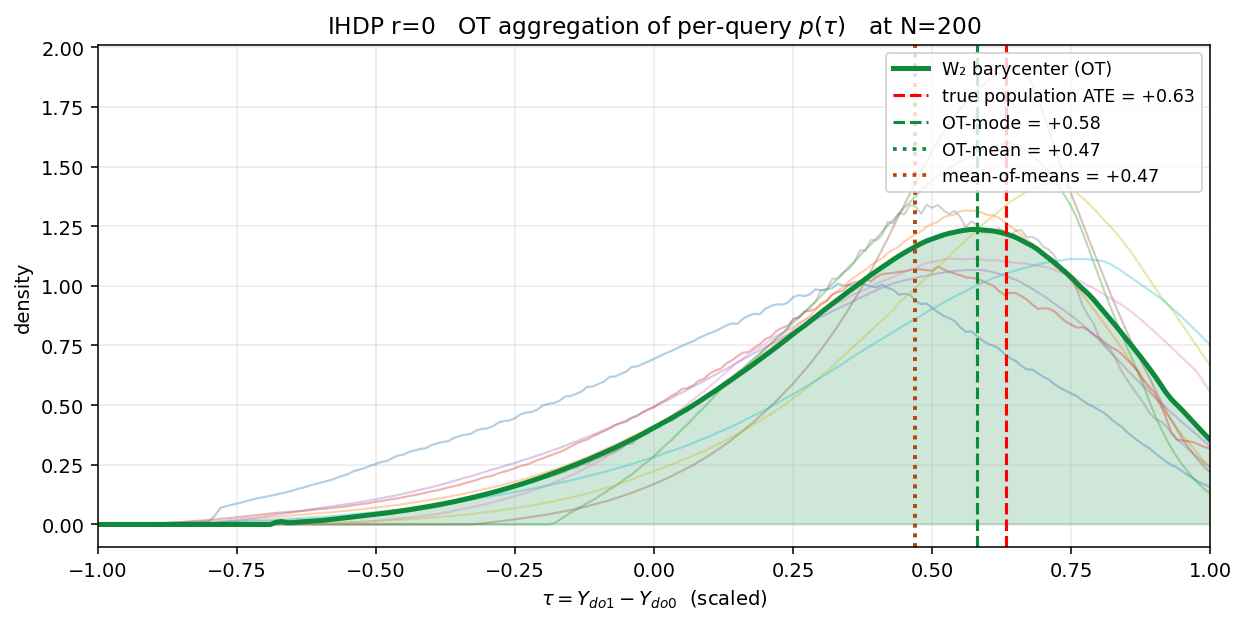
\includegraphics[width=\textwidth]{../../benchmarks/plots/ihdp_n10/ihdp_n10_ot.png}
\caption{OT aggregation on IHDP realisation $r{=}0$ with $N{=}200$
context units. Faded curves: per-query $p(\tau \mid X_i)$ from the
MALC-smoothed joint. Solid green: 2-Wasserstein barycenter. Vertical
lines: true population ATE, OT-mode, OT-mean, and the naive mean of
per-query means. OT-mode ($+0.58$) is closer to the true population ATE
($+0.63$) than either mean-based estimator ($+0.47$).}
\label{fig:ihdp-ot}
\end{figure}

\paragraph{OT-mode and OT-mean point estimates.}
From $p^{\star}$ we extract two point estimates of the population
average treatment effect $\mathrm{ATE} = \mathbb{E}_{X}[\tau(X)]$:
\begin{equation}
  \widehat{\mathrm{ATE}}_{\mathrm{OT\text{-}mode}}
  \;=\; \arg\!\max_{\tau} p^{\star}(\tau),
  \qquad
  \widehat{\mathrm{ATE}}_{\mathrm{OT\text{-}mean}}
  \;=\; \int \tau\, p^{\star}(\tau)\, d\tau.
  \label{eq:ot-point-estimates}
\end{equation}
Both are functionals of $p^{\star}$ and hence deterministic given the
per-query densities. Their empirical behaviour is reported in the main
tables.


%% -----------------------------------------------------------------------------
\subsection{Variance reduction of the joint estimator}
\label{sec:variance-reduction}

We formalise why modelling the joint distribution
$p(Y_{\mathrm{do}(0)}, Y_{\mathrm{do}(1)} \mid X)$ can strictly reduce
the variance of the treatment-effect estimate compared to modelling the
two marginals independently.
Nothing below requires a parametric assumption on the potential-outcome
distribution beyond \emph{finite second moments}. Bivariate normality
is used only to describe the Monte-Carlo simulation in
Figure~\ref{fig:variance-reduction}.

\paragraph{Setup.}
Let $(Y_{\mathrm{do}(0)}, Y_{\mathrm{do}(1)})$ be a random pair on
$\mathbb{R}^{2}$ with
$\mathbb{E}\bigl[Y_{\mathrm{do}(\ell)}\bigr] = \mu_\ell$,
$\mathrm{Var}\bigl[Y_{\mathrm{do}(\ell)}\bigr] = \sigma_\ell^{2} < \infty$
for $\ell \in \{0, 1\}$, and
$\mathrm{Corr}\bigl[Y_{\mathrm{do}(0)}, Y_{\mathrm{do}(1)}\bigr] = \rho \in [-1, 1]$.
Define the true treatment effect $\tau \coloneqq \mu_1 - \mu_0$.
Assume $N$ context units are drawn i.i.d.\ from this joint, split
equally between the two treatment arms.

\paragraph{Marginal-only estimator.}
A marginal-only estimator constructs two independent arm-specific
sample means:
\begin{equation}
  \hat{\tau}^{\,\mathrm{marg}}
  \;=\;
  \underbrace{\tfrac{1}{N/2}\!\!\sum_{i:\,T_i=1}\!Y_i}_{\hat{\mu}_1}
  \;-\;
  \underbrace{\tfrac{1}{N/2}\!\!\sum_{i:\,T_i=0}\!Y_i}_{\hat{\mu}_0}.
\end{equation}
The two summands are independent (samples in different arms are
disjoint), so
\begin{equation}
  \mathrm{Var}\bigl(\hat{\tau}^{\,\mathrm{marg}}\bigr)
  \;=\;
  \frac{\sigma_0^{2}}{N/2} + \frac{\sigma_1^{2}}{N/2}
  \;=\;
  \frac{2\,(\sigma_0^{2} + \sigma_1^{2})}{N}.
  \label{eq:var-marg}
\end{equation}
The correlation $\rho$ does not appear.

\paragraph{Joint estimator.}
A joint estimator that pairs both potential outcomes per unit gives
\begin{equation}
  \hat{\tau}^{\,\mathrm{joint}}
  \;=\;
  \frac{1}{N}\sum_{i=1}^{N}
  \bigl(Y_{\mathrm{do}(1)}(i) - Y_{\mathrm{do}(0)}(i)\bigr).
\end{equation}
By the variance of a sum,
$\mathrm{Var}(Y_{\mathrm{do}(1)} - Y_{\mathrm{do}(0)})
  = \sigma_0^{2} + \sigma_1^{2} - 2\rho\,\sigma_0\sigma_1$, whence
\begin{equation}
  \mathrm{Var}\bigl(\hat{\tau}^{\,\mathrm{joint}}\bigr)
  \;=\;
  \frac{\sigma_0^{2} + \sigma_1^{2} - 2\rho\,\sigma_0\sigma_1}{N}.
  \label{eq:var-joint}
\end{equation}

\begin{theorem}[Variance-ratio guarantee, distribution-free]
\label{thm:variance-ratio}
Under the finite-second-moment assumption above, the marginal-to-joint
variance ratio is
\begin{equation}
  R(\rho)
  \;\coloneqq\;
  \frac{\mathrm{Var}\bigl(\hat{\tau}^{\,\mathrm{marg}}\bigr)}
       {\mathrm{Var}\bigl(\hat{\tau}^{\,\mathrm{joint}}\bigr)}
  \;=\;
  \frac{2\,(\sigma_0^{2} + \sigma_1^{2})}
       {\sigma_0^{2} + \sigma_1^{2} - 2\rho\,\sigma_0\sigma_1}
  \;\;\;\underset{\sigma_0 = \sigma_1}{=}\;\;\;
  \frac{2}{1 - \rho}.
  \label{eq:ratio}
\end{equation}
The ratio $R$ is strictly increasing in $\rho$ on $[0, 1)$, satisfies
$R(0) = 2$, and diverges as $\rho \to 1^{-}$. Consequently
$\hat{\tau}^{\,\mathrm{joint}}$ strictly dominates
$\hat{\tau}^{\,\mathrm{marg}}$ in variance for every $\rho > 0$; for
$\rho < 0$ the ordering reverses.
\end{theorem}

\begin{proof}
Substitute \eqref{eq:var-marg} and \eqref{eq:var-joint} into the
definition of $R$. Monotonicity in $\rho$ follows from the sign of
$\partial R / \partial \rho > 0$ when $\rho < 1$; the limit
$R \to \infty$ as $\rho \to 1^{-}$ is the limit
$\sigma_0^{2} + \sigma_1^{2} - 2\rho\sigma_0\sigma_1 \to
(\sigma_0 - \sigma_1)^{2}$ evaluated at $\sigma_0 = \sigma_1$.
\end{proof}

\begin{corollary}[Consistency and asymptotic normality]
\label{cor:consistency-clt}
Both $\hat{\tau}^{\,\mathrm{marg}}$ and $\hat{\tau}^{\,\mathrm{joint}}$
are unbiased for $\tau$. Under the finite-second-moment assumption,
both are strongly consistent for $\tau$ as $N \to \infty$ by the law
of large numbers, with rates $\mathcal{O}_{P}(N^{-1/2})$ from the
central limit theorem. When $\sigma_0 = \sigma_1$ and $\rho > 0$,
the joint estimator has strictly smaller asymptotic variance:
$\sqrt{N}\,(\hat{\tau} - \tau) \Rightarrow \mathcal{N}(0, v(\rho))$
with $v(\rho) = 2(\sigma^{2}+\sigma^{2})$ (marginal) or
$v(\rho) = 2\sigma^{2}(1-\rho)$ (joint).
\end{corollary}

\paragraph{Extension to log-concave, exponential-family, and mixture pairs.}
Since Theorem~\ref{thm:variance-ratio} uses only the mean and covariance
matrix of the pair, it applies unchanged whenever second moments exist.
This includes: any exponential-family joint with finite variance
(Gaussian, gamma-with-correlated-parameter constructions, etc.); any
2D log-concave joint (all log-concave densities have finite moments);
and any mixture $\sum_k \pi_k q_k$ of pairs from the previous classes,
via the standard mixture identities
$\mathrm{Var}(Y) = \sum_k \pi_k(\mathrm{Var}_k + \mu_k^{2}) - \mu^{2}$
and $\mathrm{Cov}(Y_0, Y_1) = \sum_k \pi_k \mathrm{Cov}_k(Y_0, Y_1)
+ \sum_k \pi_k (\mu_{0,k} - \mu_0)(\mu_{1,k} - \mu_1)$.
In the mixture case the effective $\rho$ used in \eqref{eq:ratio}
includes both the within-component covariances and the between-component
mean shifts; a positive between-component covariation adds a
between-cluster contribution that further widens the joint's advantage
over the marginal estimator.

\paragraph{Empirical corroboration (Figure~\ref{fig:variance-reduction}).}
The Monte-Carlo simulation uses a bivariate normal with
$\sigma_0 = \sigma_1 = 1$ and $N = 50$; Theorem~\ref{thm:variance-ratio}
then predicts $R(0) = 2$, $R(0.5) = 4$, and $R(0.9) = 20$. The
empirical ratios over $10{,}000$ trials are $2.0\times$, $4.1\times$,
and $19.9\times$, matching to within Monte-Carlo error.
Bivariate normality is convenient for the simulation but is not required
by Theorem~\ref{thm:variance-ratio}: replacing the simulator with any
finite-variance joint would produce the same theoretical ratio.

%% =============================================================================
%% Bibliography stub — swap in your project's .bib file when integrating.
%% BibTeX entries for the citations used above are listed in the accompanying
%% README.md (paper/theory/README.md).
%% =============================================================================
\bibliographystyle{plainnat}
% \bibliography{refs}          % <-- point at your project .bib

\end{document}
